\NewDocumentCommand{\insertImageWithLine}{m m m m m}{
    \node[draw=#5, line width=6pt, inner sep=0] (#1) at (#2,#3) {
        \includegraphics[width=2.5cm]{#4}
    };
}

\begin{figure}[t]
    \centering
    \resizebox{1\textwidth}{!}{
        \begin{tikzpicture}
            \definecolor{custom_blue}{HTML}{40568d}
            \definecolor{custom_yellow}{HTML}{fee826}
            \definecolor{custom_purple}{HTML}{440053}
            \definecolor{custom_light_green}{HTML}{5eca61}
            \definecolor{custom_dark_green}{HTML}{22928d}

            \begin{pgfonlayer}{background}
                \node[anchor=south west,inner sep=0] (image) at (0,0) {
                    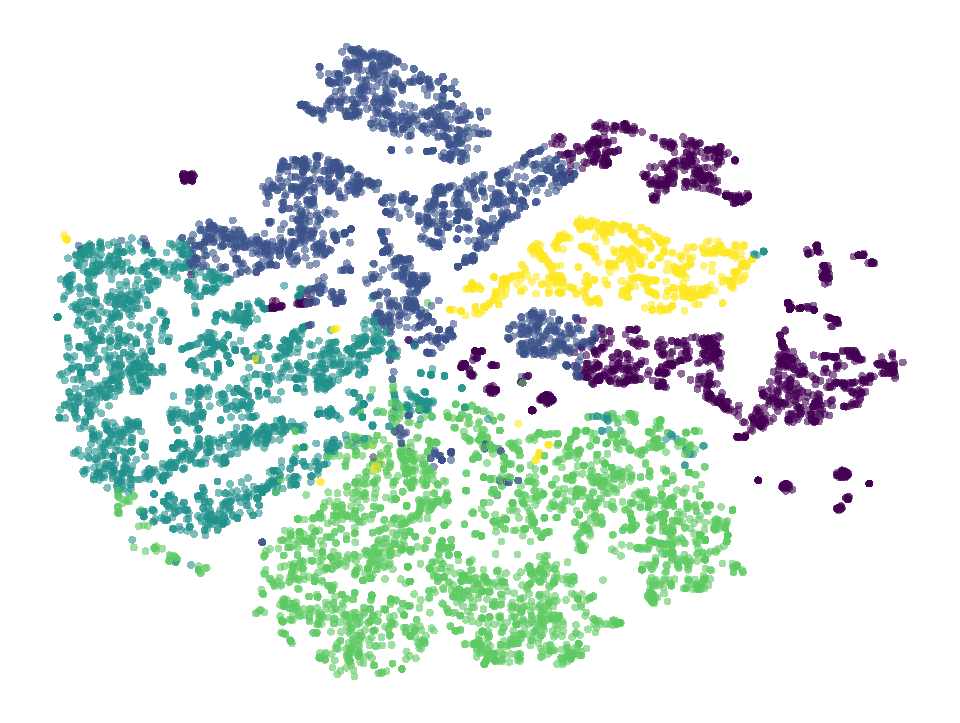
\includegraphics[]{figures/clustering_agent_representation/resources/projection_2d.pdf}
                };
            \end{pgfonlayer}

            \begin{scope}[x={(image.south east)},y={(image.north west)}]
                \node[circle, draw, inner sep=0.2cm, fill=white] (cluster_1) at (0.4,0.75) {\textbf{1}};
                \insertImageWithLine{image_1}{0.17}{0.85}{figures/clustering_agent_representation/pictures/space_invaders/5_clusters/early_game/image_1.png}{custom_blue}
                \insertImageWithLine{image_1}{0.35}{0.95}{figures/clustering_agent_representation/pictures/space_invaders/5_clusters/early_game/image_2.png}{custom_blue}

                \node[circle, draw, inner sep=0.2cm, fill=white] (cluster_2) at (0.65,0.63) {\textbf{2}};
                \insertImageWithLine{image_1}{0.57}{0.85}{figures/clustering_agent_representation/pictures/space_invaders/5_clusters/finish_right_group/image_1.png}{custom_yellow}
                \insertImageWithLine{image_1}{0.75}{0.85}{figures/clustering_agent_representation/pictures/space_invaders/5_clusters/finish_right_group/image_2.png}{custom_yellow}

                \node[circle, draw, inner sep=0.2cm, fill=white] (cluster_3) at (0.775,0.50) {\textbf{3}};
                \insertImageWithLine{image_1}{0.9}{0.55}{figures/clustering_agent_representation/pictures/space_invaders/5_clusters/catch_flying_saucer/image_1.png}{custom_purple}
                \insertImageWithLine{image_1}{0.85}{0.25}{figures/clustering_agent_representation/pictures/space_invaders/5_clusters/catch_flying_saucer/image_2.png}{custom_purple}

                \node[circle, draw, inner sep=0.2cm, fill=white] (cluster_4) at (0.525,0.25) {\textbf{4}};
                \insertImageWithLine{image_1}{0.65}{0.125}{figures/clustering_agent_representation/pictures/space_invaders/5_clusters/late_game/image_1.png}{custom_light_green}
                \insertImageWithLine{image_1}{0.40}{0.125}{figures/clustering_agent_representation/pictures/space_invaders/5_clusters/late_game/image_2.png}{custom_light_green}

                \node[circle, draw, inner sep=0.2cm, fill=white] (cluster_5) at (0.25,0.45) {\textbf{5}};
                \insertImageWithLine{image_1}{0.075}{0.50}{figures/clustering_agent_representation/pictures/space_invaders/5_clusters/mid_game/image_1.png}{custom_dark_green}
                \insertImageWithLine{image_1}{0.175}{0.20}{figures/clustering_agent_representation/pictures/space_invaders/5_clusters/mid_game/image_2.png}{custom_dark_green}
            \end{scope}

            \node (element_1) at ($(image.south) + (-7cm, -1.5cm)$) {:};
            \node[anchor=west] (element_1_text) at ($(element_1) + (0.1cm, 0cm)$) {Projection of observations into the latent space.};
            \node[anchor=east] (element_1_symbol) at ($(element_1) + (-0.1cm, 0cm)$) {
                \tikz \fill[custom_blue] (0,0) circle (3pt);
                \tikz \fill[custom_yellow] (0,0) circle (3pt);
                \tikz \fill[custom_purple] (0,0) circle (3pt);
                \tikz \fill[custom_light_green] (0,0) circle (3pt);
                \tikz \fill[custom_dark_green] (0,0) circle (3pt);
                \hspace{0.02cm}
            };

            \node (element_2) at ($(element_1) + (0cm, -0.35cm)$) {:};
            \node[anchor=west] (element_2_text) at ($(element_2) + (0.1cm, 0cm)$) {Corresponding observations to the clusters.};
            \node[anchor=east] (element_1_symbol) at ($(element_2) + (-0.1cm, 0cm)$) {
                \tikz \draw[draw=custom_blue, fill=white, line width=0.5mm] (0,0) rectangle (2mm,2mm);
                \tikz \draw[draw=custom_yellow, fill=white, line width=0.5mm] (0,0) rectangle (2mm,2mm);
                \tikz \draw[draw=custom_purple, fill=white, line width=0.5mm] (0,0) rectangle (2mm,2mm);
                \tikz \draw[draw=custom_light_green, fill=white, line width=0.5mm] (0,0) rectangle (2mm,2mm);
                \tikz \draw[draw=custom_dark_green, fill=white, line width=0.5mm] (0,0) rectangle (2mm,2mm);
            };

            \node (element_3) at ($(image.south) + (3.4cm, -1cm)$) {:};
            \node[anchor=east] (element_1_symbol) at ($(element_3) + (-0.1cm, 0cm)$) {
                \textbf{Cluster 1} \tikz \fill[custom_blue] (0,0) circle (3pt);
            };
            \node[anchor=west] (element_2_text) at ($(element_3) + (0.1cm, 0cm)$) {Few or no invaders have been neutralized.};

            \node (element_4) at ($(element_3) + (0cm, -0.35cm)$) {:};
            \node[anchor=east] (element_1_symbol) at ($(element_4) + (-0.1cm, 0cm)$) {
                \textbf{Cluster 2} \tikz \fill[custom_yellow] (0,0) circle (3pt);
            };
            \node[anchor=west] (element_2_text) at ($(element_4) + (0.1cm, 0cm)$) {The invaders on the right side are eliminated.};

            \node (element_5) at ($(element_4) + (0cm, -0.35cm)$) {:};
            \node[anchor=east] (element_1_symbol) at ($(element_5) + (-0.1cm, 0cm)$) {
                \textbf{Cluster 3} \tikz \fill[custom_purple] (0,0) circle (3pt);
            };
            \node[anchor=west] (element_2_text) at ($(element_5) + (0.1cm, 0cm)$) {Try to catch the saucer that occasionally flies.};

            \node (element_6) at ($(element_5) + (0cm, -0.35cm)$) {:};
            \node[anchor=east] (element_1_symbol) at ($(element_6) + (-0.1cm, 0cm)$) {
                \textbf{Cluster 4} \tikz \fill[custom_light_green] (0,0) circle (3pt);
            };
            \node[anchor=west] (element_2_text) at ($(element_6) + (0.1cm, 0cm)$) {Few invaders remain, moving fast near ground.};

            \node (element_7) at ($(element_6) + (0cm, -0.35cm)$) {:};
            \node[anchor=east] (element_1_symbol) at ($(element_7) + (-0.1cm, 0cm)$) {
                \textbf{Cluster 5} \tikz \fill[custom_dark_green] (0,0) circle (3pt);
            };
            \node[anchor=west] (element_2_text) at ($(element_7) + (0.1cm, 0cm)$) {Invaders descend, but their numbers are reduced.};
        \end{tikzpicture}
    }
    \caption{Two-dimensional projection of the \gls{ls} embeddings of a surrogate policy trained on Space Invaders, together with the \gls{car} clusters and their corresponding observations.}
    \label{fig:illustration_paper}
\end{figure}
